\section{Equazioni struttura stellare}\linkdest{stellarmodel}

\begin{wordonframe}{da fare: kippenhahn wiegert}
\begin{itemize}
\item strutture autogravitanti 1-62' (43). EQuilibrio idrostatico, vento stellare, stabilit\'a e pulsazioni
\item metodi numerici 77'-84(44-48)
\item esistenza e unicit\'a 85'-99'(48-56)
\item Properties of stellar matter: ideal gas with radiation, ionization, degenerate electron gas, equazione di stato, opacit\'a 102'-144'(57-78)
\item produzione energia reazioni nucleari:  146'-172'(79-92)
\item politrope 174'-190' (93-102)
\end{itemize}
\end{wordonframe}

\subsection{Struttura di equilibrio}\linkdest{stellarstructure}

\begin{frame}{Equazioni struttura di equilibrio}

\begin{align*}
&\TDy{m}{r}=\frac{1}{4\pi r^2\rho}\\
&\TDy{m}{P}=-\frac{Gm}{4\pi r^4}\overbrace{[-\frac{1}{4\pi r^2}\PtwoDy{t}{r}]}^{\tau_{hyd}=\frac{1}{2}(G\exv{\rho})\expy{-1/2}}\\
&\TDy{m}{T}=-\nabla\frac{T}{p}\frac{Gm}{4\pi r^4}\\
&\TDy{m}{L}=\epsilon-\epsilon_{\nu} \underbrace{-c_P[\TDy{t}{T}-\nad\frac{T}{P}\TDy{t}{P}]}_{-c_P\PDy{t}{T}+\frac{\delta}{\rho}\PDy{t}{P}}\\
&\TDy{t}{X_s}\frac{1}{A_s}=\sum_{production}\rho^{n_h+n_k-1}n_p\frac{X_h^{n_h}X_k^{n_k}}{A_h^{n_h}A_k^{n_k}}\frac{\exv{\sigma v}_{hk}}{m_H^{n_h+n_k-1}n_h!n_k!}\\
&-\sum_{distruction}\rho^{n_d+n_j-1}n_d\frac{X_s^{n_d}X_j^{n_j}}{A_s^{n_d}A_j^{n_j}}\frac{\exv{\sigma v}_{sj}}{m_H^{n_d+n_j-1}n_d!n_j!}
\end{align*}
\end{frame}

\begin{frame}{Conservazione massa e HE}
\begin{columns}[T]
	\begin{column}{0.5\textwidth}
\begin{align*}
&\TDy{m}{r}=\frac{1}{4\pi r^2\rho}\\
&\TDy{m}{P}=-\frac{Gm}{4\pi r^4}\overbrace{[-\frac{1}{4\pi r^2}\PtwoDy{t}{r}]}^{\tau_{hyd}=\frac{1}{2}(G\exv{\rho})\expy{-1/2}}\\
&\tau_{hyd}=\sqrt{\frac{R^3}{GM}}
\end{align*}
\end{column}\begin{column}{0.5\textwidth}
\begin{align*}
&\TDy{r}{m}=4\pi r^2\rho\\
&\TDy{r}{P}=-\frac{Gm}{r^2}\rho\overbrace{[-\rho\PtwoDy{t}{r}]}^{\tau_{hyd}=\frac{1}{2}(G\exv{\rho})\expy{-1/2}}\\
&\tau_{ff}=\sqrt{\frac{R}{g}}\\
&\tau_{exp}=R\sqrt{\frac{\rho}{P}}
\end{align*}
\end{column}
\end{columns}
Red giant: $\tau_H\approx\SI{5}{\day}$ (time for the shock to cross a supergiant star making a SNII, Cepheid); Sun: $\tau_H\approx\SI{38}{\minute}$; WD: $\tau_H\approx\SI{2}{\second}$
\end{frame}

\begin{frame}{Trasporto energia verso la superficie e gradiente termico}
\begin{columns}[T]
	\begin{column}{0.6\textwidth}
		\begin{align*}
		&\TDy{m}{T}=-\nabla\frac{T}{p}\frac{Gm}{4\pi r^4}\\
		&\nabla=\nrad=\frac{3\kappa_R}{16\pi acG}\frac{LP}{mT^4}\tag*{$\nrad\leq\nad$}\\
		&\nabla=\nad+\Delta\nabla\tag*{$\nrad>\nad-\frac{\chi_{\mu}}{\chi_T}\nmu$}
		\end{align*}
	\end{column}\begin{column}{0.4\textwidth}
		\begin{align*}
		&\TDy{r}{T}=\nabla\frac{T}{p}\TDy{r}{p}\\
		&\nabla=\TDly{P}{T}
		\end{align*}
	\end{column}
\end{columns}
\begin{align*}
&dP_{rad}=-dp=-\frac{dF_{Rad}}{c}=-\frac{F_{rad}}{c}\frac{dr}{l}=-\frac{F_{rad}}{c}\kappa_R\rho\,dr=\frac{4}{3}aT^3dT\\
&dP_{rad}(\nu)=-\frac{F_{rad}(\nu)}{c}\kappa_{\nu}\rho\,dr=\frac{4\pi}{3c}\TDy{r}{B_{\nu}(T)}\,dr\\
&B_{\nu}(T)=\frac{2h\nu^3}{c^2}\frac{1}{\exp{\frac{h\nu}{kT}}-1}
\end{align*}
\end{frame}

\begin{frame}{Equazioni struttura stellare: conservazione energia - Luminosit\'a}
\begin{columns}[T]
\begin{column}{0.4\textwidth}
\begin{align*}
&\TDy{m}{L}=\epsilon-\epsilon_{\nu} \underbrace{-c_P[\TDy{t}{T}-\nad\frac{T}{P}\TDy{t}{P}]}_{-c_P\PDy{t}{T}+\frac{\delta}{\rho}\PDy{t}{P}0-T\PDy{t}{s}}\\
&\epsilon_{gr}=-T\PDy{t}{s}=-\TDof{t}u+\frac{P}{\rho^2}\TDy{t}{\rho}\\
&\epsilon_{gr}>0\tag*{contrazione}
\end{align*}
\end{column}\begin{column}{0.6\textwidth}
\begin{align*}
&\TDy{r}{L}=4\pi r^2[\rho(\epsilon-\epsilon_{\nu})-\rho\TDof{t}u+\frac{P}{\rho}\TDy{t}{\rho}]\\
&
\end{align*}
\end{column}
\end{columns}
\end{frame}

\begin{wordonframe}{Chemical evolution: nuclear burning, diffusion and convective mixing}\linkdest{diffusion}\

\end{wordonframe}

\begin{frame}{Trasporto radiativo e convettivo: \'e valida approx idrostatica}

\end{frame}

\subsection{Relazioni approssimate per grandezze stellari fondamentali}\linkdest{omrel}

\begin{frame}{Teorema del viriale}
\begin{columns}[T]
	\begin{column}{0.5\textwidth}
		\begin{align*}
&\Omega=-\int_0^M\frac{Gm(r)}{r}\,dm\\
&\frac{1}{2}\TtwoDy{t}{I}=2E_i+\Omega\tag{T. viriale}\\
&0=\int_M\frac{3P}{\rho}\,dm(r)+\Omega\tag{stationary}\\
&E_i=\frac{1}{\gamma-1}\frac{P}{\rho}
		\end{align*}
	\end{column}\begin{column}{0.5\textwidth}
		\begin{align*}
&W=E_i+\Omega \tag{total E}\\
&\TDy{t}{W}+L=0\tag{E conservation}\\
&L=-\frac{1}{2}\dot{\Omega}=\dot{E}_i\\
&E_T=E_i+\Omega=\frac{3\gamma-4}{3(\gamma-1)}\Omega\\
&\gamma>4/3\tag{stability}
		\end{align*}
	\end{column}
\end{columns}
Nel caso in cui la contrazione gravitazionale sia l'unica fonte di energia per una massa gassosa in equilibrio idrostatico, il suo tempo di evoluzione caratteristico \'e il tempo di \kh{} $\tkh{}=\frac{\Omega}{L}\approx\frac{GM^2}{2RL}$
\end{frame}

\begin{frame}{Relazione massa, densit\'a, temperatura/ massa, peso molecolare, opacit\'a}

\end{frame}

\section{Trasporto}\linkdest{transport}

\subsection{Trasporto radiativo}\linkdest{trarad}

\begin{frame}{Trasporto radiativo}
media di rosseland
\end{frame}

\begin{frame}{Opacit\'a radiativa (analitico)}
Scattering elettronico, processi ff, fotoionizzazione; opacit\'a atmosfera: ione H-
\end{frame}

\begin{frame}{Andamento opacit\'a}
\begin{itemize}
\item Electron scattering $\rho\kappa_{\nu}=n_e\frac{8\pi}{3}(\frac{e^2}{m_ec^2})^2$ - $\sigma_T=\SI{0.66e-24}{\square\cm}$ - for $T$ maggiore di few milion K is dominant source
\item Kramers opacity: $T<\SI{e7}{\kelvin}$ - FF, BF, BB - $\kappa_R\propto\rho T\expy{-7/2}$
\end{itemize}
\end{frame}

\subsection{Conduzione}\linkdest{tracond}

\begin{frame}{Diffusione per conduzione}
stima opacit\'a per conduzione gas degenere NR
\end{frame}

\begin{frame}{Conduzione elettronica}
\begin{columns}[T]
\begin{column}{0.5\textwidth}
\begin{align*}
&F_e=-N_evl\TDy{r}{E}=-N_ekvl\TDy{r}{T}\\
&E_T\approx\frac{3}{2}kT,\ v_T\approx\sqrt{\frac{2E_T}{m}}
\end{align*}
\end{column}
\begin{column}{0.5\textwidth}
\Pelectron degenerate are forced in higher momentum state - $P_F=2\pi\hbar(\frac{3}{4\pi g})\expy{1/3}n\expy{1/3}$
\end{column}
\end{columns}
\end{frame}

\subsection{Convezione}\linkdest{traconv}

\begin{wordonframe}{Forza di archimede}
Una regione stellare \'e convettivamente stabile se una perturbazione di densit\'a infinitesima non cresce ad ampiezza finita.
\begin{equation*}\label{eq:buoyancyEOM}
\rho\PtwoDy{t}{(\Delta r)}=-g\Delta\rho=-g[\Dcvar{\TDy{r}{\rho}}{e}-\Dcvar{\TDy{r}{\rho}}{amb}]\Delta r
\end{equation*}
La forza di Archimede ha verso opposta alla perturbazione se
\begin{equation*}
[\Dcvar{\TDy{r}{\rho}}{e}-\Dcvar{\TDy{r}{\rho}}{amb}]>0
\end{equation*}
Riscrivo prima legge della termodinamica come $dq=c_P\,dT-\frac{\delta}{\rho}\,dP$
\begin{equation*}
N^2=g(\frac{1}{\Gamma_1P}\TDy{r}{P}-\frac{1}{\rho}\TDy{r}{\rho})=g(\frac{1}{\densityscale{}}-\frac{g}{c_s^2})\label{eq:bvfs}
\end{equation*}
$N^2$ rappresenta la massima frequenza sotto cui pu\'o oscillare una particella di fluido sottoposta a onde di gravit\'a mantenendo l'equilibrio di pressione con l'ambiente.
\begin{equation*}
\PtwoDy{t}{(\Delta r)}=-N^2\Delta r
\end{equation*}
che descrive un comportamento oscillatorio per $N^2>0$
\end{wordonframe}

\begin{frame}{Convective regions and temperature gradient}
\begin{columns}[T]
	\begin{column}{0.6\textwidth}
\begin{block}{Criterio di \sch e Ledoux: regioni convettive}
	\begin{align*}
	&\rho\PtwoDy{t}{(\Delta r)}=-g\Delta\rho=-g[\Dcvar{\TDy{r}{\rho}}{e}-\Dcvar{\TDy{r}{\rho}}{amb}]\Delta r\\
	&\nrad{}>\nad+\frac{\phi}{\delta}\nmu{}=\nad-\frac{\chi_{\mu}}{\chi_T}\TDly{(P)}{(\mu)}\\
	&\nrad{}>\nad\\
	&\frac{d\rho}{\rho}=\alpha\frac{dP}{P}-\delta\frac{dT}{T}+\phi\frac{d\mu}{\mu}\\
	&=-\frac{\chi_T}{\chi_{\rho}}\frac{\Delta T}{T}-\frac{\chi_{\mu}}{\chi_{\rho}}\frac{\Delta\mu(\Lambda)}{\mu}\\
	&\Delta P=0=\chi_{\rho}\frac{\Delta\rho}{\rho}+\chi_T\frac{\Delta T}{T}+\chi_{\mu}\frac{\Delta\mu}{\mu}
	\end{align*}
\end{block}
	\end{column}
	\begin{column}{0.4\textwidth}
\begin{figure}[!ht]
	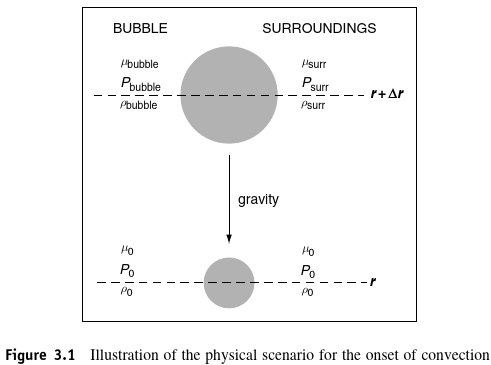
\includegraphics[trim={0cm 0cm 1cm 0cm},clip, keepaspectratio,width=0.99\textwidth]{convectivestability}\label{fig:convectivestability}
\end{figure}
\end{column}\end{columns}
\end{frame}

\begin{frame}{Mixing length: gradiente ambientale e velocit\'a elementi convettivi}
Le stelle con massa $M\leq1.1\msun{}$ hanno una regione radiativa interna mentre la parte esterna \'e convettiva. Convezione esterni $\nabla>\nad$, $v\approx1-10\si{\kilo\meter\per\second}\approx c_s$- $\nabla\to\nad{}$ in interni stellari convettivi: $\TDy{r}{T}=(1-\frac{1}{\Gamma_2})\frac{T}{P}\TDy{r}{P}$, $v\approx\SI{100}{\meter\per\second}\ll c_s$
	\begin{align*}
&F=\frac{L}{4\pi r^2}=F_{rad}+F_{con}=-\frac{4acT^3}{3\kappa\rho}\TDy{r}{T}|_{amb}+\frac{1}{2}\rho vc_p[\TDy{r}{T}|_{Ad}-\TDy{r}{T}|_{amb}]\Lambda\\
&v^2=-\frac{1}{8}g\frac{\Delta\rho}{\rho}\Lambda=\frac{1}{8}g\frac{\Lambda}{H_P}Q(\nabla-\nad),\ Q=1-\TDly{T}{\mu},\ \Lambda=\alpha H_P\\
&F_{con}^{up}=\frac{1}{2}\rho vc_PT\frac{\lambda}{H_P}(\nabla-\nad{})
\end{align*}
\begin{columns}[T]
\begin{column}{0.2\textwidth}
\begin{align*}
&f_r&=-g\Delta\rho(r)=0\tag*{r}\\
&&\propto\Delta r
\end{align*}
\end{column}
\begin{column}{0.8\textwidth}
Work done per unit volume moving bubble of $\Delta r$
\begin{align*}
&W(\Delta r)=-g\int_0^{\Delta r}\Delta\rho(\Delta r')d(\Delta r')=-\frac{1}{2}g\Delta\rho(\Delta r)\Delta r\\
&\exv{W(\Delta r)}_{\Delta r}=\frac{1}{4}W(\Lambda)=\frac{1}{2}\rho v^2
\end{align*}
\end{column}\end{columns}
%Calcolo altezza scala di pressione, flusso convettivo e gradiente ambientale in funzione della velocit\'a media degli elementi
\end{frame}

\begin{wordonframe}{EOS e $\nad{}$}
Considero un'equazione di stato generica $\rho(P,T,\mu)$ e definita tramite:
\begin{align*}
&\frac{d\rho}{\rho}=\alpha\frac{dP}{P}-\delta\frac{dT}{T}+\phi\frac{d\mu}{\mu}\\
&P=\frac{\rho\gasconstant{}T}{\mu}\quad\Rightarrow\quad\alpha=\delta=\phi=1
\end{align*}
Definisco le lunghezze caratteristiche per variazione di densit\'a e pressione:
\begin{equation*}
\densityscale{}=-\frac{dr}{d\ln{\rho}},\ H_P=-\frac{dr}{d\ln{P}}
\end{equation*}
e i gradienti termici per il blob, l'ambiente e il gradiente di composizione chimica ambientale
\begin{equation*}
\nabla=\Dcvar{\TDly{P}{T}}{amb},\ \nabla_e=\Dcvar{\TDly{P}{T}}{e},\ \nmu{}=\Dcvar{\TDly{P}{\mu}}{amb}
\end{equation*}
\end{wordonframe}

\begin{wordonframe}{EOS e EOM}
Riscrivo l'equazione del moto utilizzando l'equazione di stato per scrivere la differenza di densit\'a in termini dei gradienti termici e di composizione chimica; inoltre supponendo il moto dell'elemento in equilibrio di pressione con l'ambiente e assumendo $\nmu{}_{blob}\approx0$ risulta:
\begin{equation*}
\PtwoDy{t}{(\Delta r)}=-g\frac{\delta}{H_P}[\nabla_e-\nabla-\frac{\phi}{\delta}\nmu{}]\Delta r
\end{equation*}
\end{wordonframe}

\begin{wordonframe}{Criterio di \sch/Ledoux}
Infine per ricavare il criterio di stabilit\'a per convezione suppongo  il moto del blob adiabatico:
\begin{equation*}
dq=c_P\,dT-\frac{\delta}{\rho}\,dP
\end{equation*}
da cui risulta:
\begin{equation*}
\nabla_e=\nabla_{ad}=\frac{P\delta}{T\rho c_P}
\end{equation*}
cio\'e una regione solare \'e stabile per convezione se
\begin{equation*}
\nrad{}<\nad+\frac{\phi}{\delta}\nmu{}\label{eq:ledoux}
\end{equation*}
dove ho usato $\nabla_{amb}=\nrad{}$, cio\'e il gradiente che si ha nel caso l'energia sia trasportata dai fotoni.
\end{wordonframe}

\subsection{Teoria della mixing-length.}

\begin{wordonframe}{Convezione in esterni stellari}

In presenza di convezione il flusso di energia verso l'esterno ha una componente radiativa, determinata dal gradiente di temperatura, e una componente dominante convettiva 
\begin{equation*}\label{eq:radconvflux}
F=F_{con}+F_{rad}=\frac{\lsun{}}{4\pi r^2}
\end{equation*}

Una maggiore efficienza del trasporto convettivo di energia si riflette in una minore differenza tra il gradiente di temperature adiabatico ed effettivo.

\begin{figure}[!h]
%   \includegraphics[ width=0.99\textwidth,keepaspectratio]{proportionflux}
%   \subcaption{Profilo radiale (profondit\'a in \si{\kilo\meter}) del flusso convettivo $F_c$ rispetto al flusso totale $F$, della super-adiabaticit\'a $\nabla-\nad{}$ e regioni di ionizzazione idrogeno e $\cel{He}{4}{}{}$. Da \cite{christensen1997effects}.}\label{fluxproportion}

%\includegraphics[keepaspectratio,width=0.9\textwidth]{specificheatnablaa}
%\subcaption{Profilo radiale di $c_P$ e $\nabla_a$: si ha cambiamento di comportamento nelle regioni di ionizzazione parziale di idrogeno ed elio. Da \cite{stix91sun}.}\label{specificheatnablaa}
\end{figure}

Per determinare il gradiente di temperatura effettivo $\nabla$ uso la teoria della mixing-length:
si considera l'eccesso di calore trasportato dai blob di gas nel moto convettivo $c_P\Delta T$ rispetto all'ambiente, il cui cammino libero medio \'e la mixing-length $l_m=\alpha H_P$, che da luogo al flusso di energia
\begin{equation*}
F_{con}=\exv{\rho vc_P\Delta T}\label{eq:convectiveflux}
\end{equation*}
dove $\exv{}$ indica una media opportuna sulla sfera di raggio r. Determino il valor medio della differenza di temperatura prendendo come valore caratteristico dello spostamento del blob $\Delta r\approx\frac{l_m}{2}$:
%, considerando moti in entrambi i versi,
\begin{equation*}
\frac{\Delta T}{T}\approx\frac{1}{T}\PDy{r}{(\Delta T)}\frac{l_m}{2}=(\nabla-\nabla_e)\frac{l_m}{2}\frac{1}{H_P}\label{eq:blobambdiff}
\end{equation*}

Assumo il lavoro medio fatto dalla forza di galleggiamento per unit\'a di massa $-g\frac{\Delta\rho}{\rho}$ uguale al valore medio della forza, cio\'e la met\'a di quello alla superficie sferica data, moltiplicato lo spostamento medio $\frac{l_m}{2}$ quindi, assumendo in oltre che in media met\'a del lavoro fatto dalla forza di galleggiamento sia trasformato in energia cinetica del blob si ottiene
\begin{equation*}
v^2=g\delta(\nabla-\nabla_e)\frac{l_m^2}{8H_P}\label{eq:blobvelocity}
\end{equation*}

Infine determino gli scambi radiative del blob: il modulo del flusso radiativo \'e proporzionale al gradiente termico in direzione normale alla superficie del blob
\begin{equation*}
f=\frac{4acT^3}{3\kappa\rho}|\PDy{n}{T}|
\end{equation*}
quindi l'energia scambiata dall'intera superficie S del blob \'e $\lambda=Sf$ che determina, per la prima legge della termodinamica, una variazione di temperatura per unit\'a di tempo:
\begin{equation*}
\PDy{t}{T_e}=-\frac{\lambda}{\rho Vc_P}
\end{equation*}
indicato con $V$ il volume del blob.

La variazione della temperatura del blob per unit\'a distanza percorsa \'e quindi
\begin{equation*}
\Dcvar{\TDy{r}{T}}{e}=\Dcvar{\TDy{r}{T}}{ad}-\frac{\lambda}{\rho Vc_Pv}\label{eq:Tchangelength}
\end{equation*}
e approssimando il gradiente normale alla superficie con $\exv{\Delta T}$ ed usando le definizioni \eqref{eq:nablavitense} si ottiene:
\begin{equation*}
\frac{\nabla_e-\nad{}}{\nabla-\nabla_e}=\frac{6acT^3}{\kappa\rho^2c_Pl_mv}
\end{equation*}
Il gradiente termico ambientale $\nabla$ e del blob $\nabla_e$ sono determinati da \eqref{eq:radconvflux} e \eqref{eq:Tchangelength} inserendo le espressioni per il flusso radiativo \eqref{eq:radiativeflux} e il flusso convettivo \eqref{eq:convectiveflux}.

In figura (\subref{fluxproportion}) si mostrano l'andamento di $\nabla-\nad{}$, il profilo termico e la frazione di flusso totale trasportato dalla convezione; in figure (\subref{specificheatnablaa}) si mostrano il profilo del calore specifico per unit\'a di massa e del gradiente adiabatico.

Le 5 equazioni del flusso convettivo

Le 5 equazioni determinano completamente le variabili $F_{rad}, F_{con}, v, \nabla_e, \nabla$ in funzione di $P,T,l(r),m(r),c_P,\nad{},\nrad{},g$.

Come determino il gradiente effettivo ??

Determino $\nabla-\nabla_e$
cubic equation for $(\nabla-\nabla_e)$

\end{wordonframe}

\subsection{Approssimazione politropa}\linkdest{poly}

\begin{frame}{Trasformazioni politropiche}
\begin{block}{Gener. T. adiabatica}
	Il rapporto $\gamma=\frac{c_P}{c_V}$ costante per gas perfetto di sole particelle totalmente ionizzato.
	T. adiabatica:
	\[TV\expy{\gamma-1}=\const,\ PV\expy{\gamma}=\const,\ P\expy{1-\gamma}T\expy{\gamma}=\const\]
$0=dE-\frac{P}{\rho^2}d\rho$
Caso pi\'u generale delle trasformazioni adiabatiche: \keyword{trasformazione politropa} trasformazione quasi-statica in maniera che $c=\TDy{Q}{T}$ (calore specifico) vari in maniera assegnata. (adiabatica: $c=0$, isoterma: $c=\infty$, isometrica: $c=c_V$, ...)
\end{block}
\begin{block}{Relazione politropa - EOS}
\begin{columns}[T]
	\begin{column}{0.4\textwidth}
\begin{align*}
&\TDy{r}{P}=-\TDy{r}{\phi}\rho\\
&\frac{1}{r^2}\TDof{r}(r^2\TDy{r}{\phi})=4\pi G\rho\\
&\TDy{r}{\phi}=-\gamma K\rho\expy{\gamma-2}\TDy{r}{\rho}
\end{align*}
\end{column}
\begin{column}{0.6\textwidth}
\begin{align*}
&P=K\rho\expy{\gamma}=K\rho\expy{1+1/n}\\
&\gamma=5/3, n=3/2\tag{NR deg}\\
&\gamma=4/3, n=3\tag{R deg}\\
&\gamma=1, n=\infty\tag{isot.}\\
&\nad\approx\frac{2}{5}\tag{conv}\\
&P\propto\rho\expy{5/3}
\end{align*}
For convective exponent K varies from star to star
\end{column}\end{columns}
\end{block}
\end{frame}

\begin{frame}{Equazione Lane-Emden}
\begin{columns}[T]
	\begin{column}{0.5\textwidth}
\begin{align*}
&\rho=(\frac{-\phi}{(n+1)K})^n\tag{HE}\\
&\TtwoDy{r}{\phi}+\frac{2}{r}\TDy{r}{\phi}=4\pi G(\frac{-\phi}{(n+1)K})^n\tag{Poiss}\\
&\TtwoDy{z}{w}+\frac{2}{z}\TDy{z}{w}+w^n=0\\
&\frac{1}{z^2}\TDof{z}(z^2\TDy{z}{w})+w^n=0\tag{Lane-Emden}
\end{align*}
	\end{column}
	\begin{column}{0.5\textwidth}
		\begin{align*}
	&z=Ar\tag{new vars}\\
	&A^2=\frac{4\pi G}{(n+1)^nK^n}(-\phi_c)\expy{n-1}\\
	&=\frac{4\pi G}{(n+1)K}\rho_c\expy{\frac{n-1}{n}}\\
	&w=\frac{\phi}{\phi_c}=(\frac{\rho}{\rho_c})\expy{1/n}
		\end{align*}
\end{column}\end{columns}
\end{frame}

\begin{frame}{Strutture isoterme e modello solare}

\end{frame}

\subsection{Equazione di stato}\linkdest{eos}

\begin{wordonframe}{Schema fisico/chimico: ingredienti EOS realistiche}
\begin{itemize}
\item schema chimico: il primo considera atomi e molecole, la cui popolazione per stati eccitati e diversi gradi di ionizzazione \'e ottenuto minimizzando l'energia libera da cui sono ricavate le altre grandezze termodinamiche; utilizzando questo approccio \'e stata ricavata l'equazione di stato MHD (\cite{hummer1988equation})
\item schema fisico: nuclei ed elettroni come costituenti fondamentali interagenti tramite potenziale Coulombiano e trova le soluzione dell'equazione di Schr\"oedinger per un problema a molti corpi, questo approccio, usato per ricavare l'equazione di stato OPAL (\cite{rogers1986occupation})
\end{itemize}


Come illustrato in figura, per entrambe $\Gamma_1\approx\midfrac{5}{3}$ nell'interno solare e maggiori deviazioni si hanno nelle regioni di ionizzazione parziale degli elementi in particolare di idrogeno ed elio.
\end{wordonframe}

\begin{wordonframe}{Relazione tra $P(\rho, T)$: approx zero gas perfetto di atomi completamente ionizzati}
\begin{columns}[T]
\begin{column}{0.55\textwidth}
EOS gas perfetto di ioni ed elettroni 
\begin{equation*}
P_G=P_I+P_e=\frac{\rho}{\mu}\gasconstant{}T
\end{equation*}
Energia interna per unit\'a di massa: somma delle energie traslazionali delle particelle pesate secondo la distribuzione di equilibrio di Maxwell-Boltzmann per grammo di materia
\begin{align*}
&u=\frac{1}{\rho}\sum_i\int f^{(0)}(\vec{p}_i)\frac{p^2_i}{2m_i}\,d^3p_i\\
&=\frac{3}{2}\frac{P}{\rho}=\frac{3}{2}\frac{\gasconstant T}{\mu}
\end{align*}
\end{column}
\begin{column}{0.45\textwidth}
Peso molecolare medio: massa media in amu per particella libera
\begin{align*}
&\mu=\frac{1}{\bar{n}_HX+\bar{n}_{He}Y+\bar{n}_{Z}Z}\\
&\mu_0=\frac{1}{X+\midfrac{Y}{4}+\midfrac{Z}{\bar{A}}},\ \mu_e\approx\frac{2}{1+X}
\end{align*}
con $\bar{n}_i=\frac{1+f_i}{A_i}$ numero medio di particelle libere per unit\'a di massa atomica dovute alla specie i di peso atomico $A_i$ e $f_i$ numero medio di elettroni liberati da ione della specie i; peso atomico medio per ione $\mu_0$ ed elettrone libero (ionizzato) $\mu_e$.
\end{column}
\end{columns}
$f^{(0)}(\vec{p}_i)$: numero di particelle della specie i per unit\'a di volume con impulso in $[\vec{p}_i,\vec{p}_i+d\vec{p}_i]$
\end{wordonframe}

\begin{wordonframe}{Deviazioni dalla legge dei gas perfetti: radiazione e degenerazione elettronica}
\begin{itemize}
	\item Radiazione. Il contributo alla pressione ed energia interna per unit\'a di volume dei fotoni $P_R=\frac{a}{3}T^4$, $u_R=aT^4$, e $P-P_R=\beta P$.
	\item Degenerazione elettronica - Principio di Pauli: non pi\'u di 2 elettroni in volume di spazio delle fasi $h^3$. $n_e$ la densit\'a numerica di \Pelectron, $\psi(P,T)$ il parametro di degenerazione, tale che per $\psi\to-\infty$ si abbia la distribuzione di Boltzmann e per $\psi\to+\infty$ completa degenerazione
	\begin{align*}
	&n_e=\rho N_A\frac{1+X}{2}=\intzi{}\frac{8\pi p^2\,dp}{h^3(\exp{\frac{u_k}{KT}-\psi}+1)}=\frac{8\pi}{h^3}(2m_ekT)\expy{3/2}a(\psi)\\
	&P_e=\beta P-\rho\gasconstant{}(X+\frac{Y}{4}+\frac{Z}{\exv{A_Z}})=\frac{8\pi}{3h^3}\intzi{}p^3v(p)\frac{dp}{1+\exp{\epsilon/kT-\psi}}\\
	&U_e=\frac{8\pi}{h^3}\int_0^{\infty}\frac{p^2\epsilon(p)\,dp}{\exp{(-\psi+\midfrac{\epsilon}{KT})}+1}
	\end{align*}
\end{itemize}
\end{wordonframe}

\begin{frame}{degenerazione completa: casi limite NR e R}
\begin{align*}
&P_e=\int_{2\pi}\frac{d\Omega}{4\pi}\intzi{}dpf(p)v(p)p^2\cos{\theta}=\frac{8\pi}{3h^3}\int_0^{P_F}p^3v(p)\,dp\\
&=\frac{8\pi c}{3h^3}\int_0^{P_F}\frac{p/(m_ec)}{\sqrt{1+p^2/(m_ec)^2}}=\frac{\pi m_e^4c^5}{3h^2}f(x)\\
&U_e=\int_0^{P_F}f(p)E(p)\,dp=\frac{8\pi}{h^3}\int_0^{P_F}E(p)p^2\,dp=\frac{\pi m_e^4c^5}{3h^3}g(x)\
\end{align*}
\begin{align*}
&n_e=\frac{\rho}{\mu_em_H}=\frac{8\pi m_ec^3}{3h^3}x^3\\
&x=\frac{P_F}{m_ec}\ll1:\quad&x\gg1:\\
&P_e=\frac{8\pi m_e^4c^5}{15h^3}x^5=\frac{2}{3}U_e&P_e=\frac{2\pi m_e^4c^5}{3h^3}x^4=\frac{1}{3}U_e\\
&=\num{1.0036e13}(\frac{\rho}{\mu_e})\expy{5/3}&=\num{1.2435e15}(\frac{\rho}{\mu_e})\expy{4/3}
\end{align*}
\end{frame}

\begin{wordonframe}{Elettrostatic screening of ions: weak screening}
La principale correzione che tiene conto dell'interazioni tra particelle \'e dovuta alle interazioni coulombiane: influence EOS and nuclear rection rates.

Screening of ion i with charge $Z_ie$ ar $\vec{r_i}$ in NR dilute plasma, motion of screened ions is slow compared to screening particles: continuum static equilibrium charge distribution (\Pelectron, light ions of mean charge $Z_p$)
\begin{equation*}
\nabla^2\phi=4\pi n_ee[\exp{(\frac{e\phi}{kT})}-\exp{-\frac{Z_pe\phi}{kT}}]-4\pi\sum_iZ_ie\delta(\vec{r}-\vec{r_i})
\end{equation*}
Regime di schermaggio debole, $e\phi\ll KT$: $\phi=\sum_i\phi_i$ potenziale attorno a ione pesante isolato:
\begin{align*}
%&\nabla^2\phi=-4\pi e\sum_Z Zn_Z-4\pi e\sum_i Z_i\delta(\vec{r}-\vec{r}_i)\\
&\phi_i=\frac{Z_ie}{r_i}\exp{-\frac{r_i}{r_D}}
&\frac{1}{r_D^2}=\frac{4\pi e^2}{kT}\sum Z^2\overline{n}_Z=\frac{4\pi e^2}{kT}N_A\zeta,\ \zeta=\sum_{i}(Z_i^2+Z_i)\frac{\rho X_i}{A_i}
\end{align*}
\end{wordonframe}

\begin{wordonframe}{Elettrostatic screening of ions: energy pressure correction}
Energy required to assemble uniform shere with charge $Ze$: $U_{ee}=\int_0^{R_Z}\frac{q_r}{r}\,dq=\frac{3}{5}\frac{(Ze)^2}{R_Z}$.
Energy required to assemble uniform cloud of charge $Ze$ around Z-nucleus: $U_{eZ}=-Ze\int_0^{R_Z}\frac{dq}{r}=-\frac{3}{2}\frac{(Ze)^2}{R_Z}$
Le correzioni dovute alle interazioni coulombiane sono dovute a numero sfere ioniche per unit\'a di volume $n_Z=\frac{\rho X_Z}{A_Z}N_0$ with average potential energy per electron $\exv{-e\phi}_Z=-\frac{9}{10}\frac{(Ze)^2}{R_Z}$ that contain Z \Pelectron.
\begin{align*}
&\rho u_c=(\frac{U}{V})_e=\frac{1}{2}\phi(\vec{r})\rho_c(\vec{r})\to \frac{1}{2}\sum_ZeZ\overline{n}_Z\phi_Z=-e^3\sqrt{\frac{\pi\rho}{kT}}(N_A\zeta)\expy{\frac{3}{2}},\ P_c=\frac{1}{3}\rho u_c\\
&E_0=\frac{(U/V)_e}{n_e}=\mu_e\sum_Z\exv{-e\phi}_Z\frac{ZX_Z}{A_Z}\approx-1.3(\mu_e^2\rho)\expy{1/3}[X+0.79Y+\sum_{Z>2}\frac{Z\expy{5/3}X_Z}{A_Z}]
\end{align*}
\end{wordonframe}

\begin{frame}{Equazione di Saha e continuum depression. Ioniozzazione da pressione}
L'equazione di Saha descrive la frazione relativa di ionizzazione
\begin{align*}
&\frac{n_{r+1}}{n_r}n_e=\frac{g_{r+1}}{g_r}f_r(T)\\
&f_r(T)=2\frac{(2\pi m_ekT)\expy{3/2}}{h^3}\exp{-\chi_r/(kT)}
\end{align*}
Saha limitation:
\begin{itemize}
\item LTE: is the case when collision dominate over radiative processes
\item Decreases ionization energy with increasing density: what is called pressure ionizzation is produced by coulomb interaction of bound electron with other electron in the plasma $\chi'_Z=\chi_Z-\frac{Ze^2}{R_D}$
\end{itemize}
\end{frame}

\begin{frame}{Crystallization and Neutronization}
\begin{block}{Crystallization}
Per $\rho$ alta e $T$ bassa (WD interior: $\Gamma_c=\frac{(Ze)^2}{r_{ion}kT}\approx180$) gli ioni formano reticolo quando energia termica uguale interazione coulombiana $\frac{3}{2}kT\approx E_c$ - melting $T_m\approx\frac{Z^2e^2}{\Gamma_ck}(\frac{4\pi\rho}{3\mu_0m_H})\expy{1/3}=\num{2.3e3}Z^2\mu_0\expy{-1/3}\rho\expy{1/3}$
\end{block}
\begin{block}{Neutronization}
If \Pelectron have $E_e>E^*=c^2(m_n-m_p)\approx\SI{1.3}{\mega\ev}$ they combine with protons and form neutrons: if we put $E=E_{kin}+m_ec^2=E_F+m_ec^2=c^2(m_n-m_p)\approx\SI{1.3}{\mega\ev}$ if $E_{kin}<E_F$ l'elettrone non trova stati liberi e il neutrone non decade ($x=\frac{p_F}{m_ec}\approx2.2$).
For $\rho>\SI{4e11}{\gram\per\cubic\cm}$ we have inverse $beta$-decay:nuclei capture electron and become neutron rich - neutron drip
\end{block}
\end{frame}

\subsection{Reazioni nucleari}\linkdest{nuclearreactions}

\begin{frame}{Sezione d'urto nucleare}
schermaggio elettronico nelle stelle
\end{frame}

\begin{frame}{Catena PP}
dipendenza da T
flusso neutrini
\end{frame}

\begin{frame}{Biciclo CNO}
dipendenza da T
flusso neutrini
Modalit\'a combustione H in He: sequenza principale inferiore/superiore
\end{frame}

\begin{frame}{Combustion He}

\end{frame}

\begin{frame}{Produzione nuclei fino al Fe56}
3$\alpha$: $He4+\alpha\to C12$, $C12+\alpha\to O16$
Produzione neutroni liberi
Fusione $C12$, fotodisintegrzione $Ne20$, fusione $O16$, fotodisintegrzione $Si28$, catture $\alpha$ su nuclei fino a produzione $Fe56$
\end{frame}

\begin{frame}{Cattura neutronica: processi r e s}
picchi r e s nella nella curva universale delle abbondanze
\end{frame}

\begin{frame}{Reaction rate di fusione}
Sia $E$ l'energia cinetica nel centro di massa dei nuclei, la sezione d'urto $\sigma(E)$ di fusione \'e: $\sigma(E)=\pi\lambdabar^2*P_0(E)*S(E)$ - prodotto della sezione d'urto geometrica, della probabilit\'a di attraversamento della barriera coulombiana e del fattore astrofisico.

La lunghezza d'onda di de Broglie relativa delle particelle descrive l'indeterminazione sulla posizione nell'urto di due particelle con momento relativo p: $\lambdabar=\frac{\hbar}{p}=\frac{\hbar}{\sqrt{2mE}}$

Il fattore astrofisico $S(E)$ descrive l'interazione tra i due reagenti a livello nucleare ed \'e debolmente dipendente dall'energia lontano da risonanze.

La probabilit\'a di attraversamento della barriera coulombiana \'e:
\begin{equation}
P_0(E)=\exp{-2\pi\eta},\ \eta=\sqrt{\frac{m}{2}}\frac{Z_1Z_2e^2}{\hbar E\expy{\frac{1}{2}}}
\end{equation}
Sezione d'urto per i nuclei di carica $Z_1$, $Z_2$ e m massa ridotta:
\begin{equation}
\sigma(E)=\frac{S(E)}{E}\exp{-2\pi\eta}\label{eq:fusioncrosssection}
\end{equation}
\end{frame}

\begin{frame}{Gamow Peak}
Per determinare $\exv{\sigma v}$ - media sulla distribuzione di Maxwell-Boltzmann $f(E)dE\propto\frac{E\expy{\frac{1}{2}}}{(kT)\expy{\frac{3}{2}}}\exp{-\frac{E}{kT}}\,dE$ - uso il fatto che l'integrando
\begin{equation*}
S(E)\exp{-\frac{E}{kT}-\frac{b}{\sqrt{E}}}\label{eq:reactionrateM}
\end{equation*}
ha forma approssimativamente gaussiana il cui massimo $E_G$, energia pi\'u probabile di reazione, e FWHM sono:
\begin{equation*}
E_G=\SI{5.665}{\kilo\ev} A\expy{\frac{1}{3}}T_7\expy{\frac{2}{3}},\ \Delta E=4.249\si{\kilo\ev}W\expy{\frac{1}{6}}T_7\expy{\frac{5}{6}}
\end{equation*}
posto $W=Z_i^2Z_j^2A=Z_i^2Z_j^2\frac{A_iA_j}{A_i+A_j}$
\begin{equation*}
\exv{\sigma v}\propto b\expy{1/3}T\expy{-2/3}\exp{-\frac{b\expy{2/3}}{t\expy{1/3}}}
\end{equation*}
\end{frame}

\begin{frame}{Energy production per unit mass}
\begin{equation*}
\epsilon_{ij}(\rho,T,X_i)=Q_{ij}\frac{n_in_j}{\rho(1+\delta_{ij})}\lambda_{ij}=\frac{1}{1+\delta_{ij}}Q_{ij}\frac{\rho N_A^2X_jX_k}{{A_iA_j}}\exv{\sigma v}_{ij}
\end{equation*}
dove $Q_{ij}$ \'e l'energia liberata per reazione tra nucleo di specie i e j e $\exv{\sigma v}_{ij}$ \'e il rate di reazione per coppia di particelle; $X_i$ indica la frazione in  massa della specie i
\begin{columns}[T]
\begin{column}{0.5\textwidth}
\begin{align*}
&PP\ \exv{\sigma v}\propto T\expy{3.9}\ E_C=\SI{0.55}{\mega\ev}\\
&P^{14}N\ \exv{\sigma v}\propto T\expy{20}\ E_C=\SI{2.27}{\mega\ev}\\
&\alpha+^{12}C\ \exv{\sigma v}\propto T\expy{42}\ E_C=\SI{3.43}{\mega\ev}\\
&^{16}O+^{16}O\ \exv{\sigma v}\propto T\expy{182}\ E_C=\SI{14.07}{\mega\ev}
\end{align*}
\end{column}
\begin{column}{0.5\textwidth}
\begin{align*}
&E_C\approx Z_1Z_2\si{\mega\ev}
\end{align*}
\end{column}
\end{columns}
\end{frame}

\section{Ordini di grandezza}

\begin{frame}{Energia interna}
\begin{equation*}
E_i=\int_0^Mu\,dm=\frac{3}{2}\int_M\frac{P}{\rho}\,dm\label{eq:traslintenergy}
\end{equation*}
\end{frame}

\section{Metodi per integrazione equazioni di struttura e raccordo con modelli dell'atmosfera stellare}\linkdest{nummod}

\subsection{4 Structure ODE with boundary conditions}\linkdest{fourODE}

\begin{frame}{Equazioni struttura di equilibrio}
\begin{align*}
&\TDy{m}{r}=\frac{1}{4\pi r^2\rho}\\
&\TDy{m}{P}=-\frac{Gm}{4\pi r^4}\overbrace{[-\frac{1}{4\pi r^2}\PtwoDy{t}{r}]}^{\tau_{hyd}}\\
&\TDy{m}{T}=-\nabla\frac{T}{p}\frac{Gm}{4\pi r^4}\\
&\TDy{m}{L}=\epsilon-\epsilon_{\nu} \underbrace{-c_P[\TDy{t}{T}-\nad\frac{T}{P}\TDy{t}{P}]}_{-c_P\PDy{t}{T}+\frac{\delta}{\rho}\PDy{t}{P}: \tkh}\\
&\TDy{t}{X_s}\frac{1}{A_s}=\sum_{production}\rho^{n_h+n_k-1}n_p\frac{X_h^{n_h}X_k^{n_k}}{A_h^{n_h}A_k^{n_k}}\frac{\exv{\sigma v}_{hk}}{m_H^{n_h+n_k-1}n_h!n_k!}\\
&-\sum_{distruction}\rho^{n_d+n_j-1}n_d\frac{X_s^{n_d}X_j^{n_j}}{A_s^{n_d}A_j^{n_j}}\frac{\exv{\sigma v}_{sj}}{m_H^{n_d+n_j-1}n_d!n_j!}
\end{align*}
\end{frame}

\begin{frame}{Equazioni struttura di equilibrio: condizioni al bordo}
\begin{itemize}
\item Le 4+I equazioni determinano $r$, $P$, $T$, $L$, $X_s$ specificata la massa e composizione iniziale (omogenea)
\item $\tau_n\gg\tkh\gg\tau_{dyn}$: solve 4 structure equations at time t - do time step $\Delta t$ and determine new composition - solve structure at $t+\Delta t$ with new composition
\item Solution of 4 structure equations require 4 boundary condition: 2 at surface (atmospere model without diffusion approx, PP geometry), parametri $\rho_c,T_c$; 2 at center (via Taylor expansion for $m=m'$)
\end{itemize}
\begin{columns}[T]
\begin{column}{0.65\textwidth}
\begin{align*}
&r=(\frac{3}{4\pi\rho_c})\expy{1/3}{m'}\expy{1/3}\\
&P=P_c-\frac{3G}{8\pi}(\frac{4\pi\rho_c}{3})\expy{4/3}{m'}\expy{2/3}\\
&L=\epsilon_cm'\\
&T^4=T_c^4-\frac{1}{2ac}(\frac{3}{4\pi})\expy{2/3}\kappa_c\epsilon_c\rho_c\expy{4/3}{m'}\expy{2/3}\tag*{rad}\\
&\ln{T}=\ln{T_c}-(\frac{\pi}{6})\expy{1/3}G\frac{{\nad}_c\rho_c\expy{4/3}}{P_c}{m'}\expy{2/3}\tag*{con}
\end{align*}
\end{column}
\begin{column}{0.35\textwidth}
At surface $m=M$, $L=L_s$, atmospheric model for $P$, $T$ - atmosphere defined by $g=\frac{GM}{R^2}$, $T_e$, composition: provides $P_s$ at $\tau$ where diffusion approx. starts to be valid
\end{column}
\end{columns}
\end{frame}

\begin{frame}{Simplified atmosferic model: grey atmosphere}
Atmosphere model: usually PP geometry and solve HE equation using non grey radiative transport and EOS and convection if needed
\begin{align*}
&\TDy{\tau}{P}=\frac{g}{\kappa}\tag*{HE using $\tau$ as indip var}\\
&T^4=\frac{3}{4}T_e^4(\tau+\frac{2}{3})\tag*{or solar $T(\tau)$ empirical relation}
\end{align*}
integration from $\tau\approx0$ where $T\approx0$, $P\approx0$ down to $\tau=\frac{2}{3}$ where $T=T_e$ - using shooting method.
\end{frame}

\begin{frame}{Chemical mixing: diffusion and convection}

\end{frame}

\subsection{Metodo di Henyey: modelli evolutivi}

\begin{frame}{Metodo di Henyey $[96]$}
N mass-shell with boundaries at $m_j$ $m_1=0,m_2=m',\ldots,m_N=M$
\begin{columns}[T]
\begin{column}{0.5\textwidth}
\begin{align*}
&\frac{r_{j+1}-r_j}{m_{j+1}-m_j}=\frac{1}{4\pi r_{j+1/2}^2\rho_{j+1/2}}\\
&\frac{P_{j+1}-P_j}{m_{j+1}-m_j}=-\frac{Gm_{j+1/2}}{4\pi r_{j+1/2}}\\
&\frac{L_{j+1}-L_j}{m_{j+1}-m_j}=\epsilon_n(T_{j+1/2},\rho_{j+1/2},X_{s,j+1/2})+!!!\\
&\frac{T_{j+1}-T_j}{m_{j+1}-m_j}=-\frac{T_{j+1/2}}{P_{j+1/2}}\nabla_{j+1/2}\frac{Gm_{j+1/2}}{4\pi r^4_{j+1/2}}
\end{align*}
\end{column}
\begin{column}{0.5\textwidth}
\begin{align*}
&(Y^1=r, y^2=P, y^3=T, y^4=L)\\
&E_j^{i=1,\ldots,4}=\frac{y_{j+1}^i-y^i_j}{m_{j+1}^i-m^i_j}\\
&-f_i(y_{j+1/2}^1,\ldots,y_{j+1/2}^4)=0
\end{align*}
$j=2,\ldots,N-2$: 4N-8 vincoli e le condizioni al bordo
\begin{align*}
&J=N: S_1=y_N^2-f_S(y_N^1,y_N^4)=0\\
&S_2:y^3_N-g_S(y_N^1,y_N^4)=0\\
&j=1: C_i(y^1_2,y_2^2,y_2^3,y_2^4,y_1^2,y_1^3)=0\\
&y_1^1=y_1^4=0
\end{align*}
\end{column}
\end{columns}
$4N-2$ equazioni in $4N-2$ incognite
\end{frame}

\begin{frame}{Metodo di Henyey: solve system of algebraic equations}
\'A la Newton-Rapshon - Trial solution (solution at step $t-\Delta t$): $(S_i)_1\neq0$, $(C_i)_1\neq0$, $(E_i^j)_1\neq0$ so we have to find correction to trial solution $(y_i^j)_2=(y_i^j)_1+\delta y_i^j$ - by Taylor expansion we can express $\delta S_i$, $\delta C_i$, $\delta E^i_j$ as function of the unknown small correction:
\begin{align*}
&(S_i)_1+\delta S_i=0, (C_i)_1+\delta C_i=0, (E_i^j)_1+\delta E_i^j=0\\
&\left\{\begin{array}{l}\TDy{y_N^1}{S_i}\delta y_N^1+\TDy{y_N^2}{S_i}\delta y_N^2+\TDy{y_N^3}{S_i}\delta y_N^3+\TDy{y_N^4}{S_i}\delta y_N^4=-(S_i)_1\\
\TDy{y_2^1}{C_i}\delta y_2^1+\ldots+\TDy{y_2^4}{C_i}\delta y_2^4+\TDy{y_1^2}{C_i}\delta y_1^2+\TDy{y_1^3}{C_i}\delta y_1^3=-(C_i)_1\\
\TDy{y_j^1}{E_j^i}\delta y_j^1+\ldots+\TDy{y_j^4}{E_j^i}\delta y_j^4+\TDy{y_{j+1}^1}{E_j^i}\delta y_{j+1}^1\ldots+\TDy{y_{j+1}^4}{E_j^i}\delta y_{j+1}^4=-(E_j^i)_1\\
\end{array}\right.
\end{align*}
con $i=1,\ldots,4$, $j=2,\ldots,N$: sistema algebrico di $4N-2$ equazioni in $4N-2$ $\delta y_j^i$ incognite ha matrice dei coefficienti (\keyword{Henyey matrix}) non-zero only near the diagonal e determinante non nullo - soluzione con metodi algebrici standard - fisso $\epsilon>0$ accuratezza con cui voglio risolvere le equazioni della struttura stellare e ripeto la procedura finch\'e $S_i<\epsilon$, $C_i<\epsilon$ - local errors doesn't propagate to other mesh
\end{frame}

\subsection{Metodo di shooting: soluzione primo modello stellare con condizioni al bordo}\linkdest{shooting}

\begin{frame}{Step temporale e problema modello iniziale}
Step temporale $\Delta t$: uso metodo di Henyey per determinare le nuove abbondanze with I equations as I elements accounted for.
\keyword{Problem of first model}: i) Turn on $\epsilon_g$ within few models ii) Initial model of evolutionary sequence is evaluated with \keyword{shooting method}
starting from outer mesh with 4 boundary conditions for $T_e$, $L_s$, $P_s$, $R$ and using first order approx. $y_j^i=y_{j\pm1}^i+\TDy{m}{y_{j\pm1}}\,dm$: we determine $(y_f^i)_{surf}$ until some mesh f midway between center and surface and then integrate from centerup to $j=f$ using central trial conditions - we have $(y_f^i)_{center}\neq(y_f^i)_{surf}$ and have to correct trial central boundary conditions
\begin{columns}[T]
	\begin{column}{0.5\textwidth}
\begin{align*}
&\Delta(y_f^i)_{surf}=\TDy{y_N^1}{(y^i_f)_{surf}}\delta y_N^1+\TDy{y_N^4}{(y^i_f)_{surf}}\delta y_N^4\\
&\Delta(y_f^i)_{center}=\TDy{y_1^2}{(y^i_f)_{center}}\delta y_1^2+\TDy{y_1^3}{(y^i_f)_{center}}\delta y_1^3
\end{align*}
	\end{column}
	\begin{column}{0.5\textwidth}
correzione ai 4 valori al contorno $\delta y_N^1=\delta R$, $\delta y_N^4=\delta L_s$ e $\delta y_1^2=P_c$, $\delta y_1^3=T_c$ found solving \[-\Delta_f=\Delta(y_f^i)_{center}-\Delta(y_f^i)_{surf}\]
	\end{column}
\end{columns}
Fails in advanced stages when structure has strong gradient - In massive stars late phases we can't ignore acceleration term
\end{frame}